% Created by tikzDevice version 0.12.6 on 2024-03-28 14:16:27
% !TEX encoding = UTF-8 Unicode
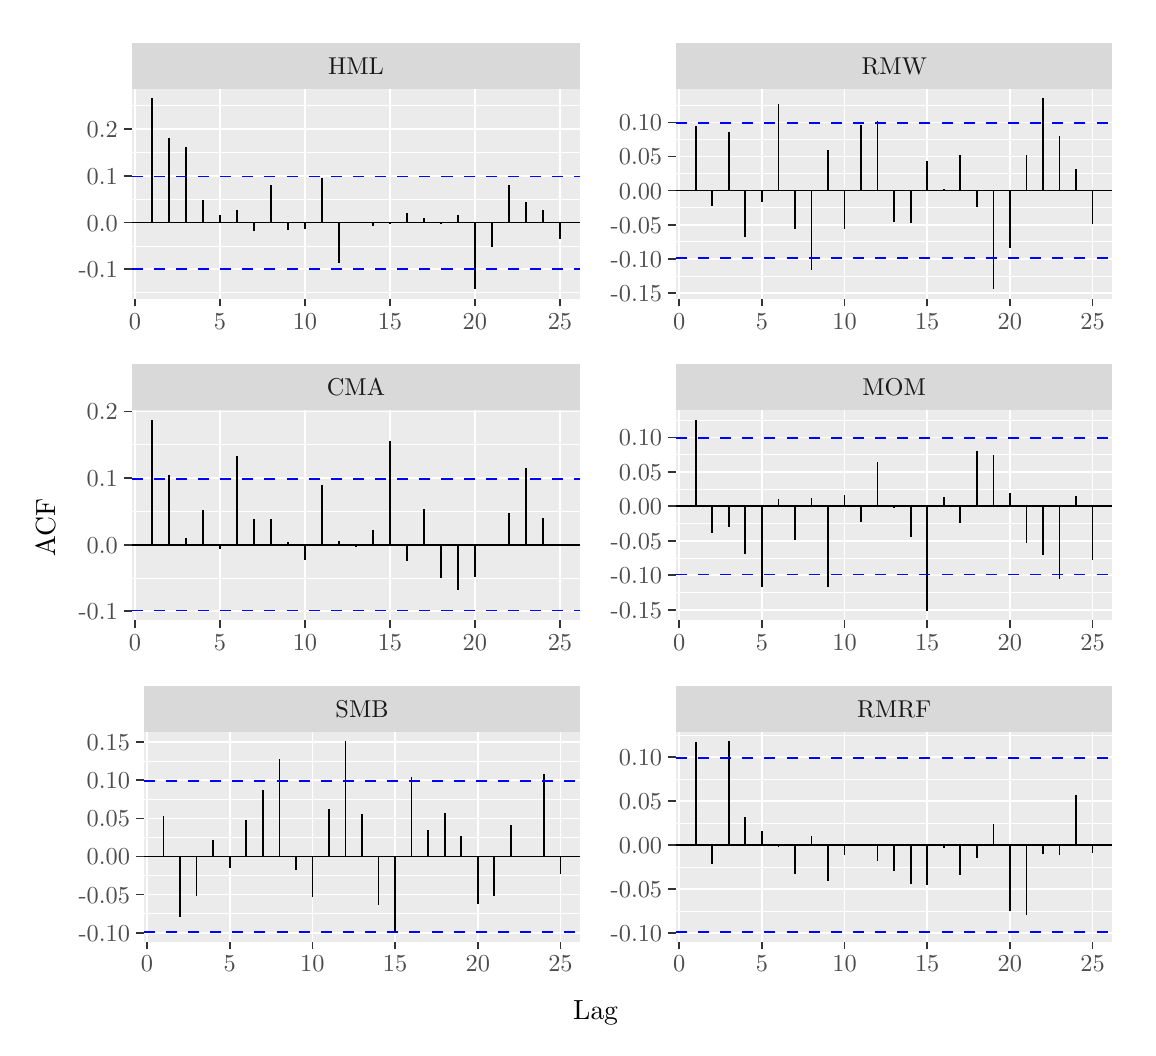
\begin{tikzpicture}[x=1pt,y=1pt]
\definecolor{fillColor}{RGB}{255,255,255}
\path[use as bounding box,fill=fillColor,fill opacity=0.00] (0,0) rectangle (397.48,361.35);
\begin{scope}
\path[clip] ( 12.91,245.20) rectangle (205.20,361.35);
\definecolor{drawColor}{RGB}{255,255,255}
\definecolor{fillColor}{RGB}{255,255,255}

\path[draw=drawColor,line width= 0.6pt,line join=round,line cap=round,fill=fillColor] ( 12.91,245.20) rectangle (205.20,361.35);
\end{scope}
\begin{scope}
\path[clip] ( 37.53,263.42) rectangle (199.70,339.28);
\definecolor{fillColor}{gray}{0.92}

\path[fill=fillColor] ( 37.53,263.42) rectangle (199.70,339.28);
\definecolor{drawColor}{RGB}{255,255,255}

\path[draw=drawColor,line width= 0.3pt,line join=round] ( 37.53,265.60) --
	(199.70,265.60);

\path[draw=drawColor,line width= 0.3pt,line join=round] ( 37.53,282.47) --
	(199.70,282.47);

\path[draw=drawColor,line width= 0.3pt,line join=round] ( 37.53,299.34) --
	(199.70,299.34);

\path[draw=drawColor,line width= 0.3pt,line join=round] ( 37.53,316.21) --
	(199.70,316.21);

\path[draw=drawColor,line width= 0.3pt,line join=round] ( 37.53,333.08) --
	(199.70,333.08);

\path[draw=drawColor,line width= 0.6pt,line join=round] ( 37.53,274.03) --
	(199.70,274.03);

\path[draw=drawColor,line width= 0.6pt,line join=round] ( 37.53,290.90) --
	(199.70,290.90);

\path[draw=drawColor,line width= 0.6pt,line join=round] ( 37.53,307.77) --
	(199.70,307.77);

\path[draw=drawColor,line width= 0.6pt,line join=round] ( 37.53,324.64) --
	(199.70,324.64);

\path[draw=drawColor,line width= 0.6pt,line join=round] ( 38.76,263.42) --
	( 38.76,339.28);

\path[draw=drawColor,line width= 0.6pt,line join=round] ( 69.48,263.42) --
	( 69.48,339.28);

\path[draw=drawColor,line width= 0.6pt,line join=round] (100.19,263.42) --
	(100.19,339.28);

\path[draw=drawColor,line width= 0.6pt,line join=round] (130.90,263.42) --
	(130.90,339.28);

\path[draw=drawColor,line width= 0.6pt,line join=round] (161.61,263.42) --
	(161.61,339.28);

\path[draw=drawColor,line width= 0.6pt,line join=round] (192.33,263.42) --
	(192.33,339.28);
\definecolor{drawColor}{RGB}{0,0,0}

\path[draw=drawColor,line width= 0.6pt,line join=round] ( 37.53,290.90) -- (199.70,290.90);

\path[draw=drawColor,line width= 0.6pt,line join=round] ( 44.91,290.90) -- ( 44.91,335.83);

\path[draw=drawColor,line width= 0.6pt,line join=round] ( 51.05,290.90) -- ( 51.05,321.49);

\path[draw=drawColor,line width= 0.6pt,line join=round] ( 57.19,290.90) -- ( 57.19,318.10);

\path[draw=drawColor,line width= 0.6pt,line join=round] ( 63.33,290.90) -- ( 63.33,299.08);

\path[draw=drawColor,line width= 0.6pt,line join=round] ( 69.48,290.90) -- ( 69.48,293.55);

\path[draw=drawColor,line width= 0.6pt,line join=round] ( 75.62,290.90) -- ( 75.62,295.48);

\path[draw=drawColor,line width= 0.6pt,line join=round] ( 81.76,290.90) -- ( 81.76,287.70);

\path[draw=drawColor,line width= 0.6pt,line join=round] ( 87.90,290.90) -- ( 87.90,304.48);

\path[draw=drawColor,line width= 0.6pt,line join=round] ( 94.05,290.90) -- ( 94.05,288.06);

\path[draw=drawColor,line width= 0.6pt,line join=round] (100.19,290.90) -- (100.19,288.60);

\path[draw=drawColor,line width= 0.6pt,line join=round] (106.33,290.90) -- (106.33,307.12);

\path[draw=drawColor,line width= 0.6pt,line join=round] (112.47,290.90) -- (112.47,276.32);

\path[draw=drawColor,line width= 0.6pt,line join=round] (118.62,290.90) -- (118.62,291.24);

\path[draw=drawColor,line width= 0.6pt,line join=round] (124.76,290.90) -- (124.76,289.66);

\path[draw=drawColor,line width= 0.6pt,line join=round] (130.90,290.90) -- (130.90,290.23);

\path[draw=drawColor,line width= 0.6pt,line join=round] (137.04,290.90) -- (137.04,294.36);

\path[draw=drawColor,line width= 0.6pt,line join=round] (143.19,290.90) -- (143.19,292.53);

\path[draw=drawColor,line width= 0.6pt,line join=round] (149.33,290.90) -- (149.33,290.23);

\path[draw=drawColor,line width= 0.6pt,line join=round] (155.47,290.90) -- (155.47,293.65);

\path[draw=drawColor,line width= 0.6pt,line join=round] (161.61,290.90) -- (161.61,266.87);

\path[draw=drawColor,line width= 0.6pt,line join=round] (167.76,290.90) -- (167.76,281.99);

\path[draw=drawColor,line width= 0.6pt,line join=round] (173.90,290.90) -- (173.90,304.52);

\path[draw=drawColor,line width= 0.6pt,line join=round] (180.04,290.90) -- (180.04,298.22);

\path[draw=drawColor,line width= 0.6pt,line join=round] (186.18,290.90) -- (186.18,295.41);

\path[draw=drawColor,line width= 0.6pt,line join=round] (192.33,290.90) -- (192.33,284.82);
\definecolor{drawColor}{RGB}{0,0,255}

\path[draw=drawColor,line width= 0.6pt,dash pattern=on 4pt off 4pt ,line join=round] ( 37.53,274.22) -- (199.70,274.22);

\path[draw=drawColor,line width= 0.6pt,dash pattern=on 4pt off 4pt ,line join=round] ( 37.53,307.58) -- (199.70,307.58);
\end{scope}
\begin{scope}
\path[clip] ( 37.53,339.28) rectangle (199.70,355.85);
\definecolor{fillColor}{gray}{0.85}

\path[fill=fillColor] ( 37.53,339.28) rectangle (199.70,355.85);
\definecolor{drawColor}{gray}{0.10}

\node[text=drawColor,anchor=base,inner sep=0pt, outer sep=0pt, scale=  0.88] at (118.62,344.53) {HML};
\end{scope}
\begin{scope}
\path[clip] (  0.00,  0.00) rectangle (397.48,361.35);
\definecolor{drawColor}{gray}{0.20}

\path[draw=drawColor,line width= 0.6pt,line join=round] ( 38.76,260.67) --
	( 38.76,263.42);

\path[draw=drawColor,line width= 0.6pt,line join=round] ( 69.48,260.67) --
	( 69.48,263.42);

\path[draw=drawColor,line width= 0.6pt,line join=round] (100.19,260.67) --
	(100.19,263.42);

\path[draw=drawColor,line width= 0.6pt,line join=round] (130.90,260.67) --
	(130.90,263.42);

\path[draw=drawColor,line width= 0.6pt,line join=round] (161.61,260.67) --
	(161.61,263.42);

\path[draw=drawColor,line width= 0.6pt,line join=round] (192.33,260.67) --
	(192.33,263.42);
\end{scope}
\begin{scope}
\path[clip] (  0.00,  0.00) rectangle (397.48,361.35);
\definecolor{drawColor}{gray}{0.30}

\node[text=drawColor,anchor=base,inner sep=0pt, outer sep=0pt, scale=  0.88] at ( 38.76,252.41) {0};

\node[text=drawColor,anchor=base,inner sep=0pt, outer sep=0pt, scale=  0.88] at ( 69.48,252.41) {5};

\node[text=drawColor,anchor=base,inner sep=0pt, outer sep=0pt, scale=  0.88] at (100.19,252.41) {10};

\node[text=drawColor,anchor=base,inner sep=0pt, outer sep=0pt, scale=  0.88] at (130.90,252.41) {15};

\node[text=drawColor,anchor=base,inner sep=0pt, outer sep=0pt, scale=  0.88] at (161.61,252.41) {20};

\node[text=drawColor,anchor=base,inner sep=0pt, outer sep=0pt, scale=  0.88] at (192.33,252.41) {25};
\end{scope}
\begin{scope}
\path[clip] (  0.00,  0.00) rectangle (397.48,361.35);
\definecolor{drawColor}{gray}{0.30}

\node[text=drawColor,anchor=base east,inner sep=0pt, outer sep=0pt, scale=  0.88] at ( 32.58,271.00) {-0.1};

\node[text=drawColor,anchor=base east,inner sep=0pt, outer sep=0pt, scale=  0.88] at ( 32.58,287.87) {0.0};

\node[text=drawColor,anchor=base east,inner sep=0pt, outer sep=0pt, scale=  0.88] at ( 32.58,304.74) {0.1};

\node[text=drawColor,anchor=base east,inner sep=0pt, outer sep=0pt, scale=  0.88] at ( 32.58,321.61) {0.2};
\end{scope}
\begin{scope}
\path[clip] (  0.00,  0.00) rectangle (397.48,361.35);
\definecolor{drawColor}{gray}{0.20}

\path[draw=drawColor,line width= 0.6pt,line join=round] ( 34.78,274.03) --
	( 37.53,274.03);

\path[draw=drawColor,line width= 0.6pt,line join=round] ( 34.78,290.90) --
	( 37.53,290.90);

\path[draw=drawColor,line width= 0.6pt,line join=round] ( 34.78,307.77) --
	( 37.53,307.77);

\path[draw=drawColor,line width= 0.6pt,line join=round] ( 34.78,324.64) --
	( 37.53,324.64);
\end{scope}
\begin{scope}
\path[clip] (205.20,245.20) rectangle (397.48,361.35);
\definecolor{drawColor}{RGB}{255,255,255}
\definecolor{fillColor}{RGB}{255,255,255}

\path[draw=drawColor,line width= 0.6pt,line join=round,line cap=round,fill=fillColor] (205.20,245.20) rectangle (397.48,361.35);
\end{scope}
\begin{scope}
\path[clip] (234.22,263.42) rectangle (391.98,339.28);
\definecolor{fillColor}{gray}{0.92}

\path[fill=fillColor] (234.22,263.42) rectangle (391.98,339.28);
\definecolor{drawColor}{RGB}{255,255,255}

\path[draw=drawColor,line width= 0.3pt,line join=round] (234.22,271.64) --
	(391.98,271.64);

\path[draw=drawColor,line width= 0.3pt,line join=round] (234.22,283.97) --
	(391.98,283.97);

\path[draw=drawColor,line width= 0.3pt,line join=round] (234.22,296.29) --
	(391.98,296.29);

\path[draw=drawColor,line width= 0.3pt,line join=round] (234.22,308.62) --
	(391.98,308.62);

\path[draw=drawColor,line width= 0.3pt,line join=round] (234.22,320.94) --
	(391.98,320.94);

\path[draw=drawColor,line width= 0.3pt,line join=round] (234.22,333.27) --
	(391.98,333.27);

\path[draw=drawColor,line width= 0.6pt,line join=round] (234.22,265.48) --
	(391.98,265.48);

\path[draw=drawColor,line width= 0.6pt,line join=round] (234.22,277.80) --
	(391.98,277.80);

\path[draw=drawColor,line width= 0.6pt,line join=round] (234.22,290.13) --
	(391.98,290.13);

\path[draw=drawColor,line width= 0.6pt,line join=round] (234.22,302.46) --
	(391.98,302.46);

\path[draw=drawColor,line width= 0.6pt,line join=round] (234.22,314.78) --
	(391.98,314.78);

\path[draw=drawColor,line width= 0.6pt,line join=round] (234.22,327.11) --
	(391.98,327.11);

\path[draw=drawColor,line width= 0.6pt,line join=round] (235.42,263.42) --
	(235.42,339.28);

\path[draw=drawColor,line width= 0.6pt,line join=round] (265.30,263.42) --
	(265.30,339.28);

\path[draw=drawColor,line width= 0.6pt,line join=round] (295.18,263.42) --
	(295.18,339.28);

\path[draw=drawColor,line width= 0.6pt,line join=round] (325.05,263.42) --
	(325.05,339.28);

\path[draw=drawColor,line width= 0.6pt,line join=round] (354.93,263.42) --
	(354.93,339.28);

\path[draw=drawColor,line width= 0.6pt,line join=round] (384.81,263.42) --
	(384.81,339.28);
\definecolor{drawColor}{RGB}{0,0,0}

\path[draw=drawColor,line width= 0.6pt,line join=round] (234.22,302.46) -- (391.98,302.46);

\path[draw=drawColor,line width= 0.6pt,line join=round] (241.39,302.46) -- (241.39,325.99);

\path[draw=drawColor,line width= 0.6pt,line join=round] (247.37,302.46) -- (247.37,296.86);

\path[draw=drawColor,line width= 0.6pt,line join=round] (253.34,302.46) -- (253.34,323.74);

\path[draw=drawColor,line width= 0.6pt,line join=round] (259.32,302.46) -- (259.32,285.78);

\path[draw=drawColor,line width= 0.6pt,line join=round] (265.30,302.46) -- (265.30,298.36);

\path[draw=drawColor,line width= 0.6pt,line join=round] (271.27,302.46) -- (271.27,333.59);

\path[draw=drawColor,line width= 0.6pt,line join=round] (277.25,302.46) -- (277.25,288.76);

\path[draw=drawColor,line width= 0.6pt,line join=round] (283.22,302.46) -- (283.22,273.76);

\path[draw=drawColor,line width= 0.6pt,line join=round] (289.20,302.46) -- (289.20,317.10);

\path[draw=drawColor,line width= 0.6pt,line join=round] (295.18,302.46) -- (295.18,288.64);

\path[draw=drawColor,line width= 0.6pt,line join=round] (301.15,302.46) -- (301.15,326.00);

\path[draw=drawColor,line width= 0.6pt,line join=round] (307.13,302.46) -- (307.13,327.77);

\path[draw=drawColor,line width= 0.6pt,line join=round] (313.10,302.46) -- (313.10,291.11);

\path[draw=drawColor,line width= 0.6pt,line join=round] (319.08,302.46) -- (319.08,290.89);

\path[draw=drawColor,line width= 0.6pt,line join=round] (325.05,302.46) -- (325.05,313.15);

\path[draw=drawColor,line width= 0.6pt,line join=round] (331.03,302.46) -- (331.03,303.15);

\path[draw=drawColor,line width= 0.6pt,line join=round] (337.01,302.46) -- (337.01,315.32);

\path[draw=drawColor,line width= 0.6pt,line join=round] (342.98,302.46) -- (342.98,296.53);

\path[draw=drawColor,line width= 0.6pt,line join=round] (348.96,302.46) -- (348.96,266.87);

\path[draw=drawColor,line width= 0.6pt,line join=round] (354.93,302.46) -- (354.93,281.58);

\path[draw=drawColor,line width= 0.6pt,line join=round] (360.91,302.46) -- (360.91,315.46);

\path[draw=drawColor,line width= 0.6pt,line join=round] (366.89,302.46) -- (366.89,335.83);

\path[draw=drawColor,line width= 0.6pt,line join=round] (372.86,302.46) -- (372.86,322.16);

\path[draw=drawColor,line width= 0.6pt,line join=round] (378.84,302.46) -- (378.84,310.37);

\path[draw=drawColor,line width= 0.6pt,line join=round] (384.81,302.46) -- (384.81,290.56);
\definecolor{drawColor}{RGB}{0,0,255}

\path[draw=drawColor,line width= 0.6pt,dash pattern=on 4pt off 4pt ,line join=round] (234.22,278.08) -- (391.98,278.08);

\path[draw=drawColor,line width= 0.6pt,dash pattern=on 4pt off 4pt ,line join=round] (234.22,326.83) -- (391.98,326.83);
\end{scope}
\begin{scope}
\path[clip] (234.22,339.28) rectangle (391.98,355.85);
\definecolor{fillColor}{gray}{0.85}

\path[fill=fillColor] (234.22,339.28) rectangle (391.98,355.85);
\definecolor{drawColor}{gray}{0.10}

\node[text=drawColor,anchor=base,inner sep=0pt, outer sep=0pt, scale=  0.88] at (313.10,344.53) {RMW};
\end{scope}
\begin{scope}
\path[clip] (  0.00,  0.00) rectangle (397.48,361.35);
\definecolor{drawColor}{gray}{0.20}

\path[draw=drawColor,line width= 0.6pt,line join=round] (235.42,260.67) --
	(235.42,263.42);

\path[draw=drawColor,line width= 0.6pt,line join=round] (265.30,260.67) --
	(265.30,263.42);

\path[draw=drawColor,line width= 0.6pt,line join=round] (295.18,260.67) --
	(295.18,263.42);

\path[draw=drawColor,line width= 0.6pt,line join=round] (325.05,260.67) --
	(325.05,263.42);

\path[draw=drawColor,line width= 0.6pt,line join=round] (354.93,260.67) --
	(354.93,263.42);

\path[draw=drawColor,line width= 0.6pt,line join=round] (384.81,260.67) --
	(384.81,263.42);
\end{scope}
\begin{scope}
\path[clip] (  0.00,  0.00) rectangle (397.48,361.35);
\definecolor{drawColor}{gray}{0.30}

\node[text=drawColor,anchor=base,inner sep=0pt, outer sep=0pt, scale=  0.88] at (235.42,252.41) {0};

\node[text=drawColor,anchor=base,inner sep=0pt, outer sep=0pt, scale=  0.88] at (265.30,252.41) {5};

\node[text=drawColor,anchor=base,inner sep=0pt, outer sep=0pt, scale=  0.88] at (295.18,252.41) {10};

\node[text=drawColor,anchor=base,inner sep=0pt, outer sep=0pt, scale=  0.88] at (325.05,252.41) {15};

\node[text=drawColor,anchor=base,inner sep=0pt, outer sep=0pt, scale=  0.88] at (354.93,252.41) {20};

\node[text=drawColor,anchor=base,inner sep=0pt, outer sep=0pt, scale=  0.88] at (384.81,252.41) {25};
\end{scope}
\begin{scope}
\path[clip] (  0.00,  0.00) rectangle (397.48,361.35);
\definecolor{drawColor}{gray}{0.30}

\node[text=drawColor,anchor=base east,inner sep=0pt, outer sep=0pt, scale=  0.88] at (229.27,262.45) {-0.15};

\node[text=drawColor,anchor=base east,inner sep=0pt, outer sep=0pt, scale=  0.88] at (229.27,274.77) {-0.10};

\node[text=drawColor,anchor=base east,inner sep=0pt, outer sep=0pt, scale=  0.88] at (229.27,287.10) {-0.05};

\node[text=drawColor,anchor=base east,inner sep=0pt, outer sep=0pt, scale=  0.88] at (229.27,299.42) {0.00};

\node[text=drawColor,anchor=base east,inner sep=0pt, outer sep=0pt, scale=  0.88] at (229.27,311.75) {0.05};

\node[text=drawColor,anchor=base east,inner sep=0pt, outer sep=0pt, scale=  0.88] at (229.27,324.08) {0.10};
\end{scope}
\begin{scope}
\path[clip] (  0.00,  0.00) rectangle (397.48,361.35);
\definecolor{drawColor}{gray}{0.20}

\path[draw=drawColor,line width= 0.6pt,line join=round] (231.47,265.48) --
	(234.22,265.48);

\path[draw=drawColor,line width= 0.6pt,line join=round] (231.47,277.80) --
	(234.22,277.80);

\path[draw=drawColor,line width= 0.6pt,line join=round] (231.47,290.13) --
	(234.22,290.13);

\path[draw=drawColor,line width= 0.6pt,line join=round] (231.47,302.46) --
	(234.22,302.46);

\path[draw=drawColor,line width= 0.6pt,line join=round] (231.47,314.78) --
	(234.22,314.78);

\path[draw=drawColor,line width= 0.6pt,line join=round] (231.47,327.11) --
	(234.22,327.11);
\end{scope}
\begin{scope}
\path[clip] ( 12.91,129.06) rectangle (205.20,245.20);
\definecolor{drawColor}{RGB}{255,255,255}
\definecolor{fillColor}{RGB}{255,255,255}

\path[draw=drawColor,line width= 0.6pt,line join=round,line cap=round,fill=fillColor] ( 12.91,129.06) rectangle (205.20,245.20);
\end{scope}
\begin{scope}
\path[clip] ( 37.53,147.28) rectangle (199.70,223.13);
\definecolor{fillColor}{gray}{0.92}

\path[fill=fillColor] ( 37.53,147.28) rectangle (199.70,223.13);
\definecolor{drawColor}{RGB}{255,255,255}

\path[draw=drawColor,line width= 0.3pt,line join=round] ( 37.53,162.49) --
	(199.70,162.49);

\path[draw=drawColor,line width= 0.3pt,line join=round] ( 37.53,186.57) --
	(199.70,186.57);

\path[draw=drawColor,line width= 0.3pt,line join=round] ( 37.53,210.65) --
	(199.70,210.65);

\path[draw=drawColor,line width= 0.6pt,line join=round] ( 37.53,150.45) --
	(199.70,150.45);

\path[draw=drawColor,line width= 0.6pt,line join=round] ( 37.53,174.53) --
	(199.70,174.53);

\path[draw=drawColor,line width= 0.6pt,line join=round] ( 37.53,198.61) --
	(199.70,198.61);

\path[draw=drawColor,line width= 0.6pt,line join=round] ( 37.53,222.68) --
	(199.70,222.68);

\path[draw=drawColor,line width= 0.6pt,line join=round] ( 38.76,147.28) --
	( 38.76,223.13);

\path[draw=drawColor,line width= 0.6pt,line join=round] ( 69.48,147.28) --
	( 69.48,223.13);

\path[draw=drawColor,line width= 0.6pt,line join=round] (100.19,147.28) --
	(100.19,223.13);

\path[draw=drawColor,line width= 0.6pt,line join=round] (130.90,147.28) --
	(130.90,223.13);

\path[draw=drawColor,line width= 0.6pt,line join=round] (161.61,147.28) --
	(161.61,223.13);

\path[draw=drawColor,line width= 0.6pt,line join=round] (192.33,147.28) --
	(192.33,223.13);
\definecolor{drawColor}{RGB}{0,0,0}

\path[draw=drawColor,line width= 0.6pt,line join=round] ( 37.53,174.53) -- (199.70,174.53);

\path[draw=drawColor,line width= 0.6pt,line join=round] ( 44.91,174.53) -- ( 44.91,219.68);

\path[draw=drawColor,line width= 0.6pt,line join=round] ( 51.05,174.53) -- ( 51.05,199.77);

\path[draw=drawColor,line width= 0.6pt,line join=round] ( 57.19,174.53) -- ( 57.19,177.12);

\path[draw=drawColor,line width= 0.6pt,line join=round] ( 63.33,174.53) -- ( 63.33,187.08);

\path[draw=drawColor,line width= 0.6pt,line join=round] ( 69.48,174.53) -- ( 69.48,173.10);

\path[draw=drawColor,line width= 0.6pt,line join=round] ( 75.62,174.53) -- ( 75.62,206.74);

\path[draw=drawColor,line width= 0.6pt,line join=round] ( 81.76,174.53) -- ( 81.76,183.67);

\path[draw=drawColor,line width= 0.6pt,line join=round] ( 87.90,174.53) -- ( 87.90,183.64);

\path[draw=drawColor,line width= 0.6pt,line join=round] ( 94.05,174.53) -- ( 94.05,175.46);

\path[draw=drawColor,line width= 0.6pt,line join=round] (100.19,174.53) -- (100.19,168.87);

\path[draw=drawColor,line width= 0.6pt,line join=round] (106.33,174.53) -- (106.33,196.01);

\path[draw=drawColor,line width= 0.6pt,line join=round] (112.47,174.53) -- (112.47,175.73);

\path[draw=drawColor,line width= 0.6pt,line join=round] (118.62,174.53) -- (118.62,173.69);

\path[draw=drawColor,line width= 0.6pt,line join=round] (124.76,174.53) -- (124.76,179.90);

\path[draw=drawColor,line width= 0.6pt,line join=round] (130.90,174.53) -- (130.90,211.86);

\path[draw=drawColor,line width= 0.6pt,line join=round] (137.04,174.53) -- (137.04,168.52);

\path[draw=drawColor,line width= 0.6pt,line join=round] (143.19,174.53) -- (143.19,187.31);

\path[draw=drawColor,line width= 0.6pt,line join=round] (149.33,174.53) -- (149.33,162.62);

\path[draw=drawColor,line width= 0.6pt,line join=round] (155.47,174.53) -- (155.47,158.12);

\path[draw=drawColor,line width= 0.6pt,line join=round] (161.61,174.53) -- (161.61,162.93);

\path[draw=drawColor,line width= 0.6pt,line join=round] (167.76,174.53) -- (167.76,174.25);

\path[draw=drawColor,line width= 0.6pt,line join=round] (173.90,174.53) -- (173.90,185.98);

\path[draw=drawColor,line width= 0.6pt,line join=round] (180.04,174.53) -- (180.04,202.32);

\path[draw=drawColor,line width= 0.6pt,line join=round] (186.18,174.53) -- (186.18,184.23);

\path[draw=drawColor,line width= 0.6pt,line join=round] (192.33,174.53) -- (192.33,174.24);
\definecolor{drawColor}{RGB}{0,0,255}

\path[draw=drawColor,line width= 0.6pt,dash pattern=on 4pt off 4pt ,line join=round] ( 37.53,150.73) -- (199.70,150.73);

\path[draw=drawColor,line width= 0.6pt,dash pattern=on 4pt off 4pt ,line join=round] ( 37.53,198.33) -- (199.70,198.33);
\end{scope}
\begin{scope}
\path[clip] ( 37.53,223.13) rectangle (199.70,239.70);
\definecolor{fillColor}{gray}{0.85}

\path[fill=fillColor] ( 37.53,223.13) rectangle (199.70,239.70);
\definecolor{drawColor}{gray}{0.10}

\node[text=drawColor,anchor=base,inner sep=0pt, outer sep=0pt, scale=  0.88] at (118.62,228.39) {CMA};
\end{scope}
\begin{scope}
\path[clip] (  0.00,  0.00) rectangle (397.48,361.35);
\definecolor{drawColor}{gray}{0.20}

\path[draw=drawColor,line width= 0.6pt,line join=round] ( 38.76,144.53) --
	( 38.76,147.28);

\path[draw=drawColor,line width= 0.6pt,line join=round] ( 69.48,144.53) --
	( 69.48,147.28);

\path[draw=drawColor,line width= 0.6pt,line join=round] (100.19,144.53) --
	(100.19,147.28);

\path[draw=drawColor,line width= 0.6pt,line join=round] (130.90,144.53) --
	(130.90,147.28);

\path[draw=drawColor,line width= 0.6pt,line join=round] (161.61,144.53) --
	(161.61,147.28);

\path[draw=drawColor,line width= 0.6pt,line join=round] (192.33,144.53) --
	(192.33,147.28);
\end{scope}
\begin{scope}
\path[clip] (  0.00,  0.00) rectangle (397.48,361.35);
\definecolor{drawColor}{gray}{0.30}

\node[text=drawColor,anchor=base,inner sep=0pt, outer sep=0pt, scale=  0.88] at ( 38.76,136.27) {0};

\node[text=drawColor,anchor=base,inner sep=0pt, outer sep=0pt, scale=  0.88] at ( 69.48,136.27) {5};

\node[text=drawColor,anchor=base,inner sep=0pt, outer sep=0pt, scale=  0.88] at (100.19,136.27) {10};

\node[text=drawColor,anchor=base,inner sep=0pt, outer sep=0pt, scale=  0.88] at (130.90,136.27) {15};

\node[text=drawColor,anchor=base,inner sep=0pt, outer sep=0pt, scale=  0.88] at (161.61,136.27) {20};

\node[text=drawColor,anchor=base,inner sep=0pt, outer sep=0pt, scale=  0.88] at (192.33,136.27) {25};
\end{scope}
\begin{scope}
\path[clip] (  0.00,  0.00) rectangle (397.48,361.35);
\definecolor{drawColor}{gray}{0.30}

\node[text=drawColor,anchor=base east,inner sep=0pt, outer sep=0pt, scale=  0.88] at ( 32.58,147.42) {-0.1};

\node[text=drawColor,anchor=base east,inner sep=0pt, outer sep=0pt, scale=  0.88] at ( 32.58,171.50) {0.0};

\node[text=drawColor,anchor=base east,inner sep=0pt, outer sep=0pt, scale=  0.88] at ( 32.58,195.58) {0.1};

\node[text=drawColor,anchor=base east,inner sep=0pt, outer sep=0pt, scale=  0.88] at ( 32.58,219.65) {0.2};
\end{scope}
\begin{scope}
\path[clip] (  0.00,  0.00) rectangle (397.48,361.35);
\definecolor{drawColor}{gray}{0.20}

\path[draw=drawColor,line width= 0.6pt,line join=round] ( 34.78,150.45) --
	( 37.53,150.45);

\path[draw=drawColor,line width= 0.6pt,line join=round] ( 34.78,174.53) --
	( 37.53,174.53);

\path[draw=drawColor,line width= 0.6pt,line join=round] ( 34.78,198.61) --
	( 37.53,198.61);

\path[draw=drawColor,line width= 0.6pt,line join=round] ( 34.78,222.68) --
	( 37.53,222.68);
\end{scope}
\begin{scope}
\path[clip] (205.20,129.06) rectangle (397.48,245.20);
\definecolor{drawColor}{RGB}{255,255,255}
\definecolor{fillColor}{RGB}{255,255,255}

\path[draw=drawColor,line width= 0.6pt,line join=round,line cap=round,fill=fillColor] (205.20,129.06) rectangle (397.48,245.20);
\end{scope}
\begin{scope}
\path[clip] (234.22,147.28) rectangle (391.98,223.13);
\definecolor{fillColor}{gray}{0.92}

\path[fill=fillColor] (234.22,147.28) rectangle (391.98,223.13);
\definecolor{drawColor}{RGB}{255,255,255}

\path[draw=drawColor,line width= 0.3pt,line join=round] (234.22,157.27) --
	(391.98,157.27);

\path[draw=drawColor,line width= 0.3pt,line join=round] (234.22,169.72) --
	(391.98,169.72);

\path[draw=drawColor,line width= 0.3pt,line join=round] (234.22,182.17) --
	(391.98,182.17);

\path[draw=drawColor,line width= 0.3pt,line join=round] (234.22,194.62) --
	(391.98,194.62);

\path[draw=drawColor,line width= 0.3pt,line join=round] (234.22,207.07) --
	(391.98,207.07);

\path[draw=drawColor,line width= 0.3pt,line join=round] (234.22,219.52) --
	(391.98,219.52);

\path[draw=drawColor,line width= 0.6pt,line join=round] (234.22,151.04) --
	(391.98,151.04);

\path[draw=drawColor,line width= 0.6pt,line join=round] (234.22,163.49) --
	(391.98,163.49);

\path[draw=drawColor,line width= 0.6pt,line join=round] (234.22,175.94) --
	(391.98,175.94);

\path[draw=drawColor,line width= 0.6pt,line join=round] (234.22,188.39) --
	(391.98,188.39);

\path[draw=drawColor,line width= 0.6pt,line join=round] (234.22,200.84) --
	(391.98,200.84);

\path[draw=drawColor,line width= 0.6pt,line join=round] (234.22,213.29) --
	(391.98,213.29);

\path[draw=drawColor,line width= 0.6pt,line join=round] (235.42,147.28) --
	(235.42,223.13);

\path[draw=drawColor,line width= 0.6pt,line join=round] (265.30,147.28) --
	(265.30,223.13);

\path[draw=drawColor,line width= 0.6pt,line join=round] (295.18,147.28) --
	(295.18,223.13);

\path[draw=drawColor,line width= 0.6pt,line join=round] (325.05,147.28) --
	(325.05,223.13);

\path[draw=drawColor,line width= 0.6pt,line join=round] (354.93,147.28) --
	(354.93,223.13);

\path[draw=drawColor,line width= 0.6pt,line join=round] (384.81,147.28) --
	(384.81,223.13);
\definecolor{drawColor}{RGB}{0,0,0}

\path[draw=drawColor,line width= 0.6pt,line join=round] (234.22,188.39) -- (391.98,188.39);

\path[draw=drawColor,line width= 0.6pt,line join=round] (241.39,188.39) -- (241.39,219.68);

\path[draw=drawColor,line width= 0.6pt,line join=round] (247.37,188.39) -- (247.37,178.60);

\path[draw=drawColor,line width= 0.6pt,line join=round] (253.34,188.39) -- (253.34,180.99);

\path[draw=drawColor,line width= 0.6pt,line join=round] (259.32,188.39) -- (259.32,171.13);

\path[draw=drawColor,line width= 0.6pt,line join=round] (265.30,188.39) -- (265.30,159.34);

\path[draw=drawColor,line width= 0.6pt,line join=round] (271.27,188.39) -- (271.27,190.92);

\path[draw=drawColor,line width= 0.6pt,line join=round] (277.25,188.39) -- (277.25,176.08);

\path[draw=drawColor,line width= 0.6pt,line join=round] (283.22,188.39) -- (283.22,191.49);

\path[draw=drawColor,line width= 0.6pt,line join=round] (289.20,188.39) -- (289.20,159.09);

\path[draw=drawColor,line width= 0.6pt,line join=round] (295.18,188.39) -- (295.18,192.59);

\path[draw=drawColor,line width= 0.6pt,line join=round] (301.15,188.39) -- (301.15,182.69);

\path[draw=drawColor,line width= 0.6pt,line join=round] (307.13,188.39) -- (307.13,204.24);

\path[draw=drawColor,line width= 0.6pt,line join=round] (313.10,188.39) -- (313.10,187.74);

\path[draw=drawColor,line width= 0.6pt,line join=round] (319.08,188.39) -- (319.08,177.20);

\path[draw=drawColor,line width= 0.6pt,line join=round] (325.05,188.39) -- (325.05,150.73);

\path[draw=drawColor,line width= 0.6pt,line join=round] (331.03,188.39) -- (331.03,191.77);

\path[draw=drawColor,line width= 0.6pt,line join=round] (337.01,188.39) -- (337.01,182.29);

\path[draw=drawColor,line width= 0.6pt,line join=round] (342.98,188.39) -- (342.98,208.47);

\path[draw=drawColor,line width= 0.6pt,line join=round] (348.96,188.39) -- (348.96,206.82);

\path[draw=drawColor,line width= 0.6pt,line join=round] (354.93,188.39) -- (354.93,193.24);

\path[draw=drawColor,line width= 0.6pt,line join=round] (360.91,188.39) -- (360.91,175.18);

\path[draw=drawColor,line width= 0.6pt,line join=round] (366.89,188.39) -- (366.89,170.87);

\path[draw=drawColor,line width= 0.6pt,line join=round] (372.86,188.39) -- (372.86,162.02);

\path[draw=drawColor,line width= 0.6pt,line join=round] (378.84,188.39) -- (378.84,192.15);

\path[draw=drawColor,line width= 0.6pt,line join=round] (384.81,188.39) -- (384.81,168.93);
\definecolor{drawColor}{RGB}{0,0,255}

\path[draw=drawColor,line width= 0.6pt,dash pattern=on 4pt off 4pt ,line join=round] (234.22,163.77) -- (391.98,163.77);

\path[draw=drawColor,line width= 0.6pt,dash pattern=on 4pt off 4pt ,line join=round] (234.22,213.01) -- (391.98,213.01);
\end{scope}
\begin{scope}
\path[clip] (234.22,223.13) rectangle (391.98,239.70);
\definecolor{fillColor}{gray}{0.85}

\path[fill=fillColor] (234.22,223.13) rectangle (391.98,239.70);
\definecolor{drawColor}{gray}{0.10}

\node[text=drawColor,anchor=base,inner sep=0pt, outer sep=0pt, scale=  0.88] at (313.10,228.39) {MOM};
\end{scope}
\begin{scope}
\path[clip] (  0.00,  0.00) rectangle (397.48,361.35);
\definecolor{drawColor}{gray}{0.20}

\path[draw=drawColor,line width= 0.6pt,line join=round] (235.42,144.53) --
	(235.42,147.28);

\path[draw=drawColor,line width= 0.6pt,line join=round] (265.30,144.53) --
	(265.30,147.28);

\path[draw=drawColor,line width= 0.6pt,line join=round] (295.18,144.53) --
	(295.18,147.28);

\path[draw=drawColor,line width= 0.6pt,line join=round] (325.05,144.53) --
	(325.05,147.28);

\path[draw=drawColor,line width= 0.6pt,line join=round] (354.93,144.53) --
	(354.93,147.28);

\path[draw=drawColor,line width= 0.6pt,line join=round] (384.81,144.53) --
	(384.81,147.28);
\end{scope}
\begin{scope}
\path[clip] (  0.00,  0.00) rectangle (397.48,361.35);
\definecolor{drawColor}{gray}{0.30}

\node[text=drawColor,anchor=base,inner sep=0pt, outer sep=0pt, scale=  0.88] at (235.42,136.27) {0};

\node[text=drawColor,anchor=base,inner sep=0pt, outer sep=0pt, scale=  0.88] at (265.30,136.27) {5};

\node[text=drawColor,anchor=base,inner sep=0pt, outer sep=0pt, scale=  0.88] at (295.18,136.27) {10};

\node[text=drawColor,anchor=base,inner sep=0pt, outer sep=0pt, scale=  0.88] at (325.05,136.27) {15};

\node[text=drawColor,anchor=base,inner sep=0pt, outer sep=0pt, scale=  0.88] at (354.93,136.27) {20};

\node[text=drawColor,anchor=base,inner sep=0pt, outer sep=0pt, scale=  0.88] at (384.81,136.27) {25};
\end{scope}
\begin{scope}
\path[clip] (  0.00,  0.00) rectangle (397.48,361.35);
\definecolor{drawColor}{gray}{0.30}

\node[text=drawColor,anchor=base east,inner sep=0pt, outer sep=0pt, scale=  0.88] at (229.27,148.01) {-0.15};

\node[text=drawColor,anchor=base east,inner sep=0pt, outer sep=0pt, scale=  0.88] at (229.27,160.46) {-0.10};

\node[text=drawColor,anchor=base east,inner sep=0pt, outer sep=0pt, scale=  0.88] at (229.27,172.91) {-0.05};

\node[text=drawColor,anchor=base east,inner sep=0pt, outer sep=0pt, scale=  0.88] at (229.27,185.36) {0.00};

\node[text=drawColor,anchor=base east,inner sep=0pt, outer sep=0pt, scale=  0.88] at (229.27,197.81) {0.05};

\node[text=drawColor,anchor=base east,inner sep=0pt, outer sep=0pt, scale=  0.88] at (229.27,210.26) {0.10};
\end{scope}
\begin{scope}
\path[clip] (  0.00,  0.00) rectangle (397.48,361.35);
\definecolor{drawColor}{gray}{0.20}

\path[draw=drawColor,line width= 0.6pt,line join=round] (231.47,151.04) --
	(234.22,151.04);

\path[draw=drawColor,line width= 0.6pt,line join=round] (231.47,163.49) --
	(234.22,163.49);

\path[draw=drawColor,line width= 0.6pt,line join=round] (231.47,175.94) --
	(234.22,175.94);

\path[draw=drawColor,line width= 0.6pt,line join=round] (231.47,188.39) --
	(234.22,188.39);

\path[draw=drawColor,line width= 0.6pt,line join=round] (231.47,200.84) --
	(234.22,200.84);

\path[draw=drawColor,line width= 0.6pt,line join=round] (231.47,213.29) --
	(234.22,213.29);
\end{scope}
\begin{scope}
\path[clip] ( 12.91, 12.91) rectangle (205.20,129.06);
\definecolor{drawColor}{RGB}{255,255,255}
\definecolor{fillColor}{RGB}{255,255,255}

\path[draw=drawColor,line width= 0.6pt,line join=round,line cap=round,fill=fillColor] ( 12.91, 12.91) rectangle (205.20,129.06);
\end{scope}
\begin{scope}
\path[clip] ( 41.93, 31.13) rectangle (199.70,106.98);
\definecolor{fillColor}{gray}{0.92}

\path[fill=fillColor] ( 41.93, 31.13) rectangle (199.70,106.98);
\definecolor{drawColor}{RGB}{255,255,255}

\path[draw=drawColor,line width= 0.3pt,line join=round] ( 41.93, 41.16) --
	(199.70, 41.16);

\path[draw=drawColor,line width= 0.3pt,line join=round] ( 41.93, 54.95) --
	(199.70, 54.95);

\path[draw=drawColor,line width= 0.3pt,line join=round] ( 41.93, 68.75) --
	(199.70, 68.75);

\path[draw=drawColor,line width= 0.3pt,line join=round] ( 41.93, 82.54) --
	(199.70, 82.54);

\path[draw=drawColor,line width= 0.3pt,line join=round] ( 41.93, 96.33) --
	(199.70, 96.33);

\path[draw=drawColor,line width= 0.6pt,line join=round] ( 41.93, 34.27) --
	(199.70, 34.27);

\path[draw=drawColor,line width= 0.6pt,line join=round] ( 41.93, 48.06) --
	(199.70, 48.06);

\path[draw=drawColor,line width= 0.6pt,line join=round] ( 41.93, 61.85) --
	(199.70, 61.85);

\path[draw=drawColor,line width= 0.6pt,line join=round] ( 41.93, 75.64) --
	(199.70, 75.64);

\path[draw=drawColor,line width= 0.6pt,line join=round] ( 41.93, 89.43) --
	(199.70, 89.43);

\path[draw=drawColor,line width= 0.6pt,line join=round] ( 41.93,103.23) --
	(199.70,103.23);

\path[draw=drawColor,line width= 0.6pt,line join=round] ( 43.13, 31.13) --
	( 43.13,106.98);

\path[draw=drawColor,line width= 0.6pt,line join=round] ( 73.01, 31.13) --
	( 73.01,106.98);

\path[draw=drawColor,line width= 0.6pt,line join=round] (102.89, 31.13) --
	(102.89,106.98);

\path[draw=drawColor,line width= 0.6pt,line join=round] (132.77, 31.13) --
	(132.77,106.98);

\path[draw=drawColor,line width= 0.6pt,line join=round] (162.65, 31.13) --
	(162.65,106.98);

\path[draw=drawColor,line width= 0.6pt,line join=round] (192.53, 31.13) --
	(192.53,106.98);
\definecolor{drawColor}{RGB}{0,0,0}

\path[draw=drawColor,line width= 0.6pt,line join=round] ( 41.93, 61.85) -- (199.70, 61.85);

\path[draw=drawColor,line width= 0.6pt,line join=round] ( 49.10, 61.85) -- ( 49.10, 76.59);

\path[draw=drawColor,line width= 0.6pt,line join=round] ( 55.08, 61.85) -- ( 55.08, 39.83);

\path[draw=drawColor,line width= 0.6pt,line join=round] ( 61.06, 61.85) -- ( 61.06, 47.43);

\path[draw=drawColor,line width= 0.6pt,line join=round] ( 67.03, 61.85) -- ( 67.03, 67.78);

\path[draw=drawColor,line width= 0.6pt,line join=round] ( 73.01, 61.85) -- ( 73.01, 57.81);

\path[draw=drawColor,line width= 0.6pt,line join=round] ( 78.98, 61.85) -- ( 78.98, 75.05);

\path[draw=drawColor,line width= 0.6pt,line join=round] ( 84.96, 61.85) -- ( 84.96, 85.87);

\path[draw=drawColor,line width= 0.6pt,line join=round] ( 90.94, 61.85) -- ( 90.94, 97.26);

\path[draw=drawColor,line width= 0.6pt,line join=round] ( 96.91, 61.85) -- ( 96.91, 56.87);

\path[draw=drawColor,line width= 0.6pt,line join=round] (102.89, 61.85) -- (102.89, 47.26);

\path[draw=drawColor,line width= 0.6pt,line join=round] (108.86, 61.85) -- (108.86, 79.07);

\path[draw=drawColor,line width= 0.6pt,line join=round] (114.84, 61.85) -- (114.84,103.54);

\path[draw=drawColor,line width= 0.6pt,line join=round] (120.82, 61.85) -- (120.82, 77.08);

\path[draw=drawColor,line width= 0.6pt,line join=round] (126.79, 61.85) -- (126.79, 44.47);

\path[draw=drawColor,line width= 0.6pt,line join=round] (132.77, 61.85) -- (132.77, 35.10);

\path[draw=drawColor,line width= 0.6pt,line join=round] (138.74, 61.85) -- (138.74, 90.68);

\path[draw=drawColor,line width= 0.6pt,line join=round] (144.72, 61.85) -- (144.72, 71.46);

\path[draw=drawColor,line width= 0.6pt,line join=round] (150.69, 61.85) -- (150.69, 77.75);

\path[draw=drawColor,line width= 0.6pt,line join=round] (156.67, 61.85) -- (156.67, 69.38);

\path[draw=drawColor,line width= 0.6pt,line join=round] (162.65, 61.85) -- (162.65, 44.72);

\path[draw=drawColor,line width= 0.6pt,line join=round] (168.62, 61.85) -- (168.62, 47.74);

\path[draw=drawColor,line width= 0.6pt,line join=round] (174.60, 61.85) -- (174.60, 73.31);

\path[draw=drawColor,line width= 0.6pt,line join=round] (180.57, 61.85) -- (180.57, 61.97);

\path[draw=drawColor,line width= 0.6pt,line join=round] (186.55, 61.85) -- (186.55, 91.61);

\path[draw=drawColor,line width= 0.6pt,line join=round] (192.53, 61.85) -- (192.53, 55.57);
\definecolor{drawColor}{RGB}{0,0,255}

\path[draw=drawColor,line width= 0.6pt,dash pattern=on 4pt off 4pt ,line join=round] ( 41.93, 34.58) -- (199.70, 34.58);

\path[draw=drawColor,line width= 0.6pt,dash pattern=on 4pt off 4pt ,line join=round] ( 41.93, 89.12) -- (199.70, 89.12);
\end{scope}
\begin{scope}
\path[clip] ( 41.93,106.98) rectangle (199.70,123.56);
\definecolor{fillColor}{gray}{0.85}

\path[fill=fillColor] ( 41.93,106.98) rectangle (199.70,123.56);
\definecolor{drawColor}{gray}{0.10}

\node[text=drawColor,anchor=base,inner sep=0pt, outer sep=0pt, scale=  0.88] at (120.82,112.24) {SMB};
\end{scope}
\begin{scope}
\path[clip] (  0.00,  0.00) rectangle (397.48,361.35);
\definecolor{drawColor}{gray}{0.20}

\path[draw=drawColor,line width= 0.6pt,line join=round] ( 43.13, 28.38) --
	( 43.13, 31.13);

\path[draw=drawColor,line width= 0.6pt,line join=round] ( 73.01, 28.38) --
	( 73.01, 31.13);

\path[draw=drawColor,line width= 0.6pt,line join=round] (102.89, 28.38) --
	(102.89, 31.13);

\path[draw=drawColor,line width= 0.6pt,line join=round] (132.77, 28.38) --
	(132.77, 31.13);

\path[draw=drawColor,line width= 0.6pt,line join=round] (162.65, 28.38) --
	(162.65, 31.13);

\path[draw=drawColor,line width= 0.6pt,line join=round] (192.53, 28.38) --
	(192.53, 31.13);
\end{scope}
\begin{scope}
\path[clip] (  0.00,  0.00) rectangle (397.48,361.35);
\definecolor{drawColor}{gray}{0.30}

\node[text=drawColor,anchor=base,inner sep=0pt, outer sep=0pt, scale=  0.88] at ( 43.13, 20.12) {0};

\node[text=drawColor,anchor=base,inner sep=0pt, outer sep=0pt, scale=  0.88] at ( 73.01, 20.12) {5};

\node[text=drawColor,anchor=base,inner sep=0pt, outer sep=0pt, scale=  0.88] at (102.89, 20.12) {10};

\node[text=drawColor,anchor=base,inner sep=0pt, outer sep=0pt, scale=  0.88] at (132.77, 20.12) {15};

\node[text=drawColor,anchor=base,inner sep=0pt, outer sep=0pt, scale=  0.88] at (162.65, 20.12) {20};

\node[text=drawColor,anchor=base,inner sep=0pt, outer sep=0pt, scale=  0.88] at (192.53, 20.12) {25};
\end{scope}
\begin{scope}
\path[clip] (  0.00,  0.00) rectangle (397.48,361.35);
\definecolor{drawColor}{gray}{0.30}

\node[text=drawColor,anchor=base east,inner sep=0pt, outer sep=0pt, scale=  0.88] at ( 36.98, 31.24) {-0.10};

\node[text=drawColor,anchor=base east,inner sep=0pt, outer sep=0pt, scale=  0.88] at ( 36.98, 45.03) {-0.05};

\node[text=drawColor,anchor=base east,inner sep=0pt, outer sep=0pt, scale=  0.88] at ( 36.98, 58.82) {0.00};

\node[text=drawColor,anchor=base east,inner sep=0pt, outer sep=0pt, scale=  0.88] at ( 36.98, 72.61) {0.05};

\node[text=drawColor,anchor=base east,inner sep=0pt, outer sep=0pt, scale=  0.88] at ( 36.98, 86.40) {0.10};

\node[text=drawColor,anchor=base east,inner sep=0pt, outer sep=0pt, scale=  0.88] at ( 36.98,100.20) {0.15};
\end{scope}
\begin{scope}
\path[clip] (  0.00,  0.00) rectangle (397.48,361.35);
\definecolor{drawColor}{gray}{0.20}

\path[draw=drawColor,line width= 0.6pt,line join=round] ( 39.18, 34.27) --
	( 41.93, 34.27);

\path[draw=drawColor,line width= 0.6pt,line join=round] ( 39.18, 48.06) --
	( 41.93, 48.06);

\path[draw=drawColor,line width= 0.6pt,line join=round] ( 39.18, 61.85) --
	( 41.93, 61.85);

\path[draw=drawColor,line width= 0.6pt,line join=round] ( 39.18, 75.64) --
	( 41.93, 75.64);

\path[draw=drawColor,line width= 0.6pt,line join=round] ( 39.18, 89.43) --
	( 41.93, 89.43);

\path[draw=drawColor,line width= 0.6pt,line join=round] ( 39.18,103.23) --
	( 41.93,103.23);
\end{scope}
\begin{scope}
\path[clip] (205.20, 12.91) rectangle (397.48,129.06);
\definecolor{drawColor}{RGB}{255,255,255}
\definecolor{fillColor}{RGB}{255,255,255}

\path[draw=drawColor,line width= 0.6pt,line join=round,line cap=round,fill=fillColor] (205.20, 12.91) rectangle (397.48,129.06);
\end{scope}
\begin{scope}
\path[clip] (234.22, 31.13) rectangle (391.98,106.98);
\definecolor{fillColor}{gray}{0.92}

\path[fill=fillColor] (234.22, 31.13) rectangle (391.98,106.98);
\definecolor{drawColor}{RGB}{255,255,255}

\path[draw=drawColor,line width= 0.3pt,line join=round] (234.22, 42.16) --
	(391.98, 42.16);

\path[draw=drawColor,line width= 0.3pt,line join=round] (234.22, 58.05) --
	(391.98, 58.05);

\path[draw=drawColor,line width= 0.3pt,line join=round] (234.22, 73.95) --
	(391.98, 73.95);

\path[draw=drawColor,line width= 0.3pt,line join=round] (234.22, 89.84) --
	(391.98, 89.84);

\path[draw=drawColor,line width= 0.3pt,line join=round] (234.22,105.73) --
	(391.98,105.73);

\path[draw=drawColor,line width= 0.6pt,line join=round] (234.22, 34.22) --
	(391.98, 34.22);

\path[draw=drawColor,line width= 0.6pt,line join=round] (234.22, 50.11) --
	(391.98, 50.11);

\path[draw=drawColor,line width= 0.6pt,line join=round] (234.22, 66.00) --
	(391.98, 66.00);

\path[draw=drawColor,line width= 0.6pt,line join=round] (234.22, 81.89) --
	(391.98, 81.89);

\path[draw=drawColor,line width= 0.6pt,line join=round] (234.22, 97.78) --
	(391.98, 97.78);

\path[draw=drawColor,line width= 0.6pt,line join=round] (235.42, 31.13) --
	(235.42,106.98);

\path[draw=drawColor,line width= 0.6pt,line join=round] (265.30, 31.13) --
	(265.30,106.98);

\path[draw=drawColor,line width= 0.6pt,line join=round] (295.18, 31.13) --
	(295.18,106.98);

\path[draw=drawColor,line width= 0.6pt,line join=round] (325.05, 31.13) --
	(325.05,106.98);

\path[draw=drawColor,line width= 0.6pt,line join=round] (354.93, 31.13) --
	(354.93,106.98);

\path[draw=drawColor,line width= 0.6pt,line join=round] (384.81, 31.13) --
	(384.81,106.98);
\definecolor{drawColor}{RGB}{0,0,0}

\path[draw=drawColor,line width= 0.6pt,line join=round] (234.22, 66.00) -- (391.98, 66.00);

\path[draw=drawColor,line width= 0.6pt,line join=round] (241.39, 66.00) -- (241.39,103.11);

\path[draw=drawColor,line width= 0.6pt,line join=round] (247.37, 66.00) -- (247.37, 59.14);

\path[draw=drawColor,line width= 0.6pt,line join=round] (253.34, 66.00) -- (253.34,103.54);

\path[draw=drawColor,line width= 0.6pt,line join=round] (259.32, 66.00) -- (259.32, 76.16);

\path[draw=drawColor,line width= 0.6pt,line join=round] (265.30, 66.00) -- (265.30, 70.92);

\path[draw=drawColor,line width= 0.6pt,line join=round] (271.27, 66.00) -- (271.27, 65.33);

\path[draw=drawColor,line width= 0.6pt,line join=round] (277.25, 66.00) -- (277.25, 55.61);

\path[draw=drawColor,line width= 0.6pt,line join=round] (283.22, 66.00) -- (283.22, 69.21);

\path[draw=drawColor,line width= 0.6pt,line join=round] (289.20, 66.00) -- (289.20, 52.93);

\path[draw=drawColor,line width= 0.6pt,line join=round] (295.18, 66.00) -- (295.18, 62.43);

\path[draw=drawColor,line width= 0.6pt,line join=round] (301.15, 66.00) -- (301.15, 66.39);

\path[draw=drawColor,line width= 0.6pt,line join=round] (307.13, 66.00) -- (307.13, 60.21);

\path[draw=drawColor,line width= 0.6pt,line join=round] (313.10, 66.00) -- (313.10, 56.61);

\path[draw=drawColor,line width= 0.6pt,line join=round] (319.08, 66.00) -- (319.08, 52.04);

\path[draw=drawColor,line width= 0.6pt,line join=round] (325.05, 66.00) -- (325.05, 51.43);

\path[draw=drawColor,line width= 0.6pt,line join=round] (331.03, 66.00) -- (331.03, 65.07);

\path[draw=drawColor,line width= 0.6pt,line join=round] (337.01, 66.00) -- (337.01, 55.17);

\path[draw=drawColor,line width= 0.6pt,line join=round] (342.98, 66.00) -- (342.98, 61.20);

\path[draw=drawColor,line width= 0.6pt,line join=round] (348.96, 66.00) -- (348.96, 73.58);

\path[draw=drawColor,line width= 0.6pt,line join=round] (354.93, 66.00) -- (354.93, 42.29);

\path[draw=drawColor,line width= 0.6pt,line join=round] (360.91, 66.00) -- (360.91, 40.73);

\path[draw=drawColor,line width= 0.6pt,line join=round] (366.89, 66.00) -- (366.89, 62.87);

\path[draw=drawColor,line width= 0.6pt,line join=round] (372.86, 66.00) -- (372.86, 62.50);

\path[draw=drawColor,line width= 0.6pt,line join=round] (378.84, 66.00) -- (378.84, 84.00);

\path[draw=drawColor,line width= 0.6pt,line join=round] (384.81, 66.00) -- (384.81, 63.28);
\definecolor{drawColor}{RGB}{0,0,255}

\path[draw=drawColor,line width= 0.6pt,dash pattern=on 4pt off 4pt ,line join=round] (234.22, 34.58) -- (391.98, 34.58);

\path[draw=drawColor,line width= 0.6pt,dash pattern=on 4pt off 4pt ,line join=round] (234.22, 97.42) -- (391.98, 97.42);
\end{scope}
\begin{scope}
\path[clip] (234.22,106.98) rectangle (391.98,123.56);
\definecolor{fillColor}{gray}{0.85}

\path[fill=fillColor] (234.22,106.98) rectangle (391.98,123.56);
\definecolor{drawColor}{gray}{0.10}

\node[text=drawColor,anchor=base,inner sep=0pt, outer sep=0pt, scale=  0.88] at (313.10,112.24) {RMRF};
\end{scope}
\begin{scope}
\path[clip] (  0.00,  0.00) rectangle (397.48,361.35);
\definecolor{drawColor}{gray}{0.20}

\path[draw=drawColor,line width= 0.6pt,line join=round] (235.42, 28.38) --
	(235.42, 31.13);

\path[draw=drawColor,line width= 0.6pt,line join=round] (265.30, 28.38) --
	(265.30, 31.13);

\path[draw=drawColor,line width= 0.6pt,line join=round] (295.18, 28.38) --
	(295.18, 31.13);

\path[draw=drawColor,line width= 0.6pt,line join=round] (325.05, 28.38) --
	(325.05, 31.13);

\path[draw=drawColor,line width= 0.6pt,line join=round] (354.93, 28.38) --
	(354.93, 31.13);

\path[draw=drawColor,line width= 0.6pt,line join=round] (384.81, 28.38) --
	(384.81, 31.13);
\end{scope}
\begin{scope}
\path[clip] (  0.00,  0.00) rectangle (397.48,361.35);
\definecolor{drawColor}{gray}{0.30}

\node[text=drawColor,anchor=base,inner sep=0pt, outer sep=0pt, scale=  0.88] at (235.42, 20.12) {0};

\node[text=drawColor,anchor=base,inner sep=0pt, outer sep=0pt, scale=  0.88] at (265.30, 20.12) {5};

\node[text=drawColor,anchor=base,inner sep=0pt, outer sep=0pt, scale=  0.88] at (295.18, 20.12) {10};

\node[text=drawColor,anchor=base,inner sep=0pt, outer sep=0pt, scale=  0.88] at (325.05, 20.12) {15};

\node[text=drawColor,anchor=base,inner sep=0pt, outer sep=0pt, scale=  0.88] at (354.93, 20.12) {20};

\node[text=drawColor,anchor=base,inner sep=0pt, outer sep=0pt, scale=  0.88] at (384.81, 20.12) {25};
\end{scope}
\begin{scope}
\path[clip] (  0.00,  0.00) rectangle (397.48,361.35);
\definecolor{drawColor}{gray}{0.30}

\node[text=drawColor,anchor=base east,inner sep=0pt, outer sep=0pt, scale=  0.88] at (229.27, 31.19) {-0.10};

\node[text=drawColor,anchor=base east,inner sep=0pt, outer sep=0pt, scale=  0.88] at (229.27, 47.08) {-0.05};

\node[text=drawColor,anchor=base east,inner sep=0pt, outer sep=0pt, scale=  0.88] at (229.27, 62.97) {0.00};

\node[text=drawColor,anchor=base east,inner sep=0pt, outer sep=0pt, scale=  0.88] at (229.27, 78.86) {0.05};

\node[text=drawColor,anchor=base east,inner sep=0pt, outer sep=0pt, scale=  0.88] at (229.27, 94.75) {0.10};
\end{scope}
\begin{scope}
\path[clip] (  0.00,  0.00) rectangle (397.48,361.35);
\definecolor{drawColor}{gray}{0.20}

\path[draw=drawColor,line width= 0.6pt,line join=round] (231.47, 34.22) --
	(234.22, 34.22);

\path[draw=drawColor,line width= 0.6pt,line join=round] (231.47, 50.11) --
	(234.22, 50.11);

\path[draw=drawColor,line width= 0.6pt,line join=round] (231.47, 66.00) --
	(234.22, 66.00);

\path[draw=drawColor,line width= 0.6pt,line join=round] (231.47, 81.89) --
	(234.22, 81.89);

\path[draw=drawColor,line width= 0.6pt,line join=round] (231.47, 97.78) --
	(234.22, 97.78);
\end{scope}
\begin{scope}
\path[clip] (  0.00,  0.00) rectangle (397.48,361.35);
\definecolor{drawColor}{RGB}{0,0,0}

\node[text=drawColor,anchor=base,inner sep=0pt, outer sep=0pt, scale=  1.00] at (205.20,  3.01) {Lag};
\end{scope}
\begin{scope}
\path[clip] (  0.00,  0.00) rectangle (397.48,361.35);
\definecolor{drawColor}{RGB}{0,0,0}

\node[text=drawColor,rotate= 90.00,anchor=base,inner sep=0pt, outer sep=0pt, scale=  1.00] at (  9.90,180.67) {ACF};
\end{scope}
\end{tikzpicture}
